\documentclass{beamer}
\usepackage{amsthm}
\usepackage{amssymb}
\usepackage{amsmath}
\usepackage{amsfonts}
\usepackage{graphicx}
\usepackage{tikz}
\usetheme{Rochester}
\usecolortheme{seahorse}
\usefonttheme{structuresmallcapsserif}
\setbeamertemplate{caption}[numbered]
\setbeamertemplate{footline}[frame number]
\usepackage{subfigure}

\title{Efficient segmentation algorithms for shark fin identification}
\subtitle{Honors project proposal}
\author{L. Cilli\'{e}, Project advisors: Dr. S. van der Walt and Prof. B. Herbst}
\date{1 August 2013}
\institute{Department of Applied Mathematics, Stellenbosch University}

\begin{document}
\maketitle
\tableofcontents[ 
currentsubsection, 
hideothersubsections, 
sectionstyle=show/hide, 
subsectionstyle=show/shaded]

\begin{frame}
\frametitle{Contents}

\end{frame}

\begin{frame}
\frametitle{Problem description and motivation}
\end{frame}

\begin{frame}
\frametitle{Examples of shark fin images}

\begin{figure}
\centering
\mbox{\subfigure[Shark fin 1]{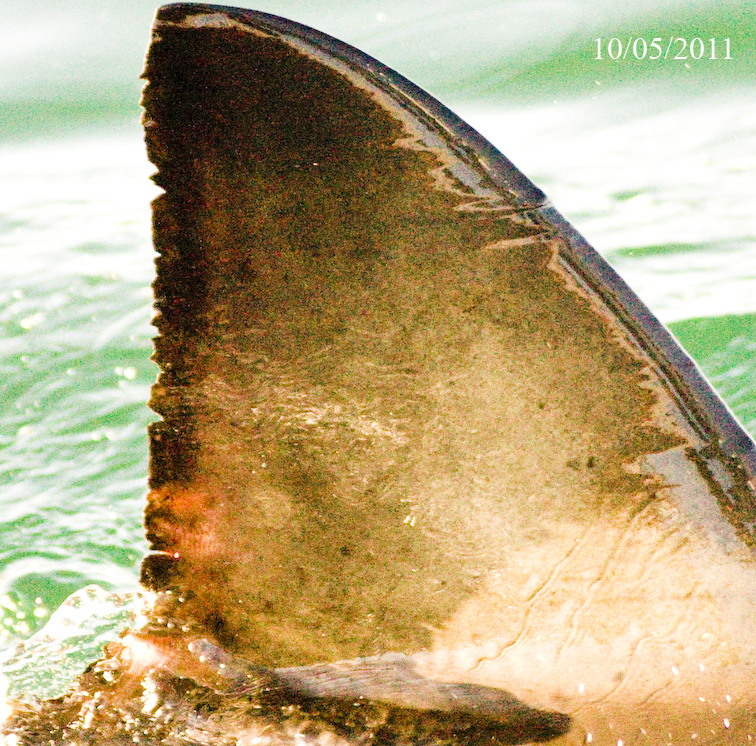
\includegraphics[width=2in]{haai1.jpg}} \quad
\subfigure[Shark fin 2]{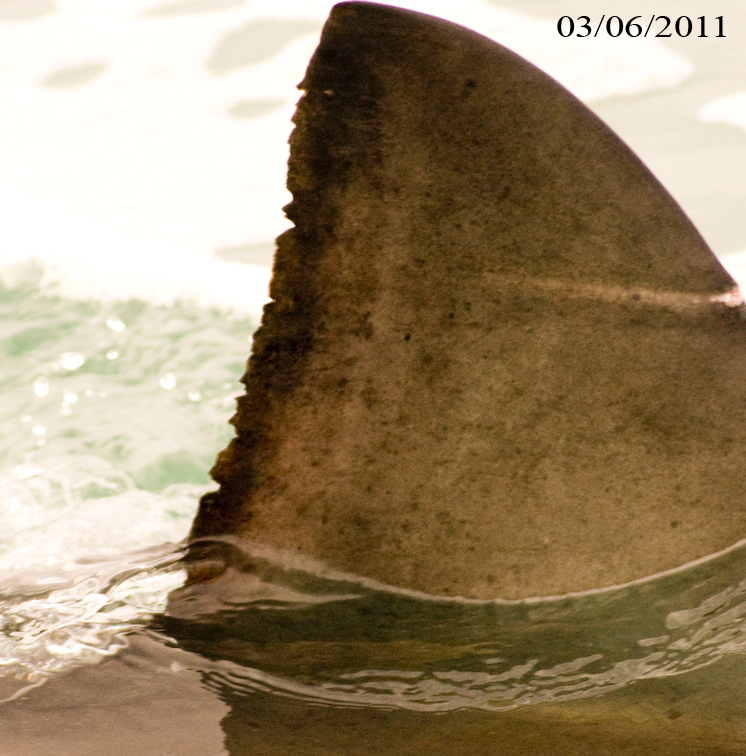
\includegraphics[width=2in]{haai2.jpg}}}
\end{figure}
\begin{figure}
\centering
\mbox{\subfigure[Shark fin 3]{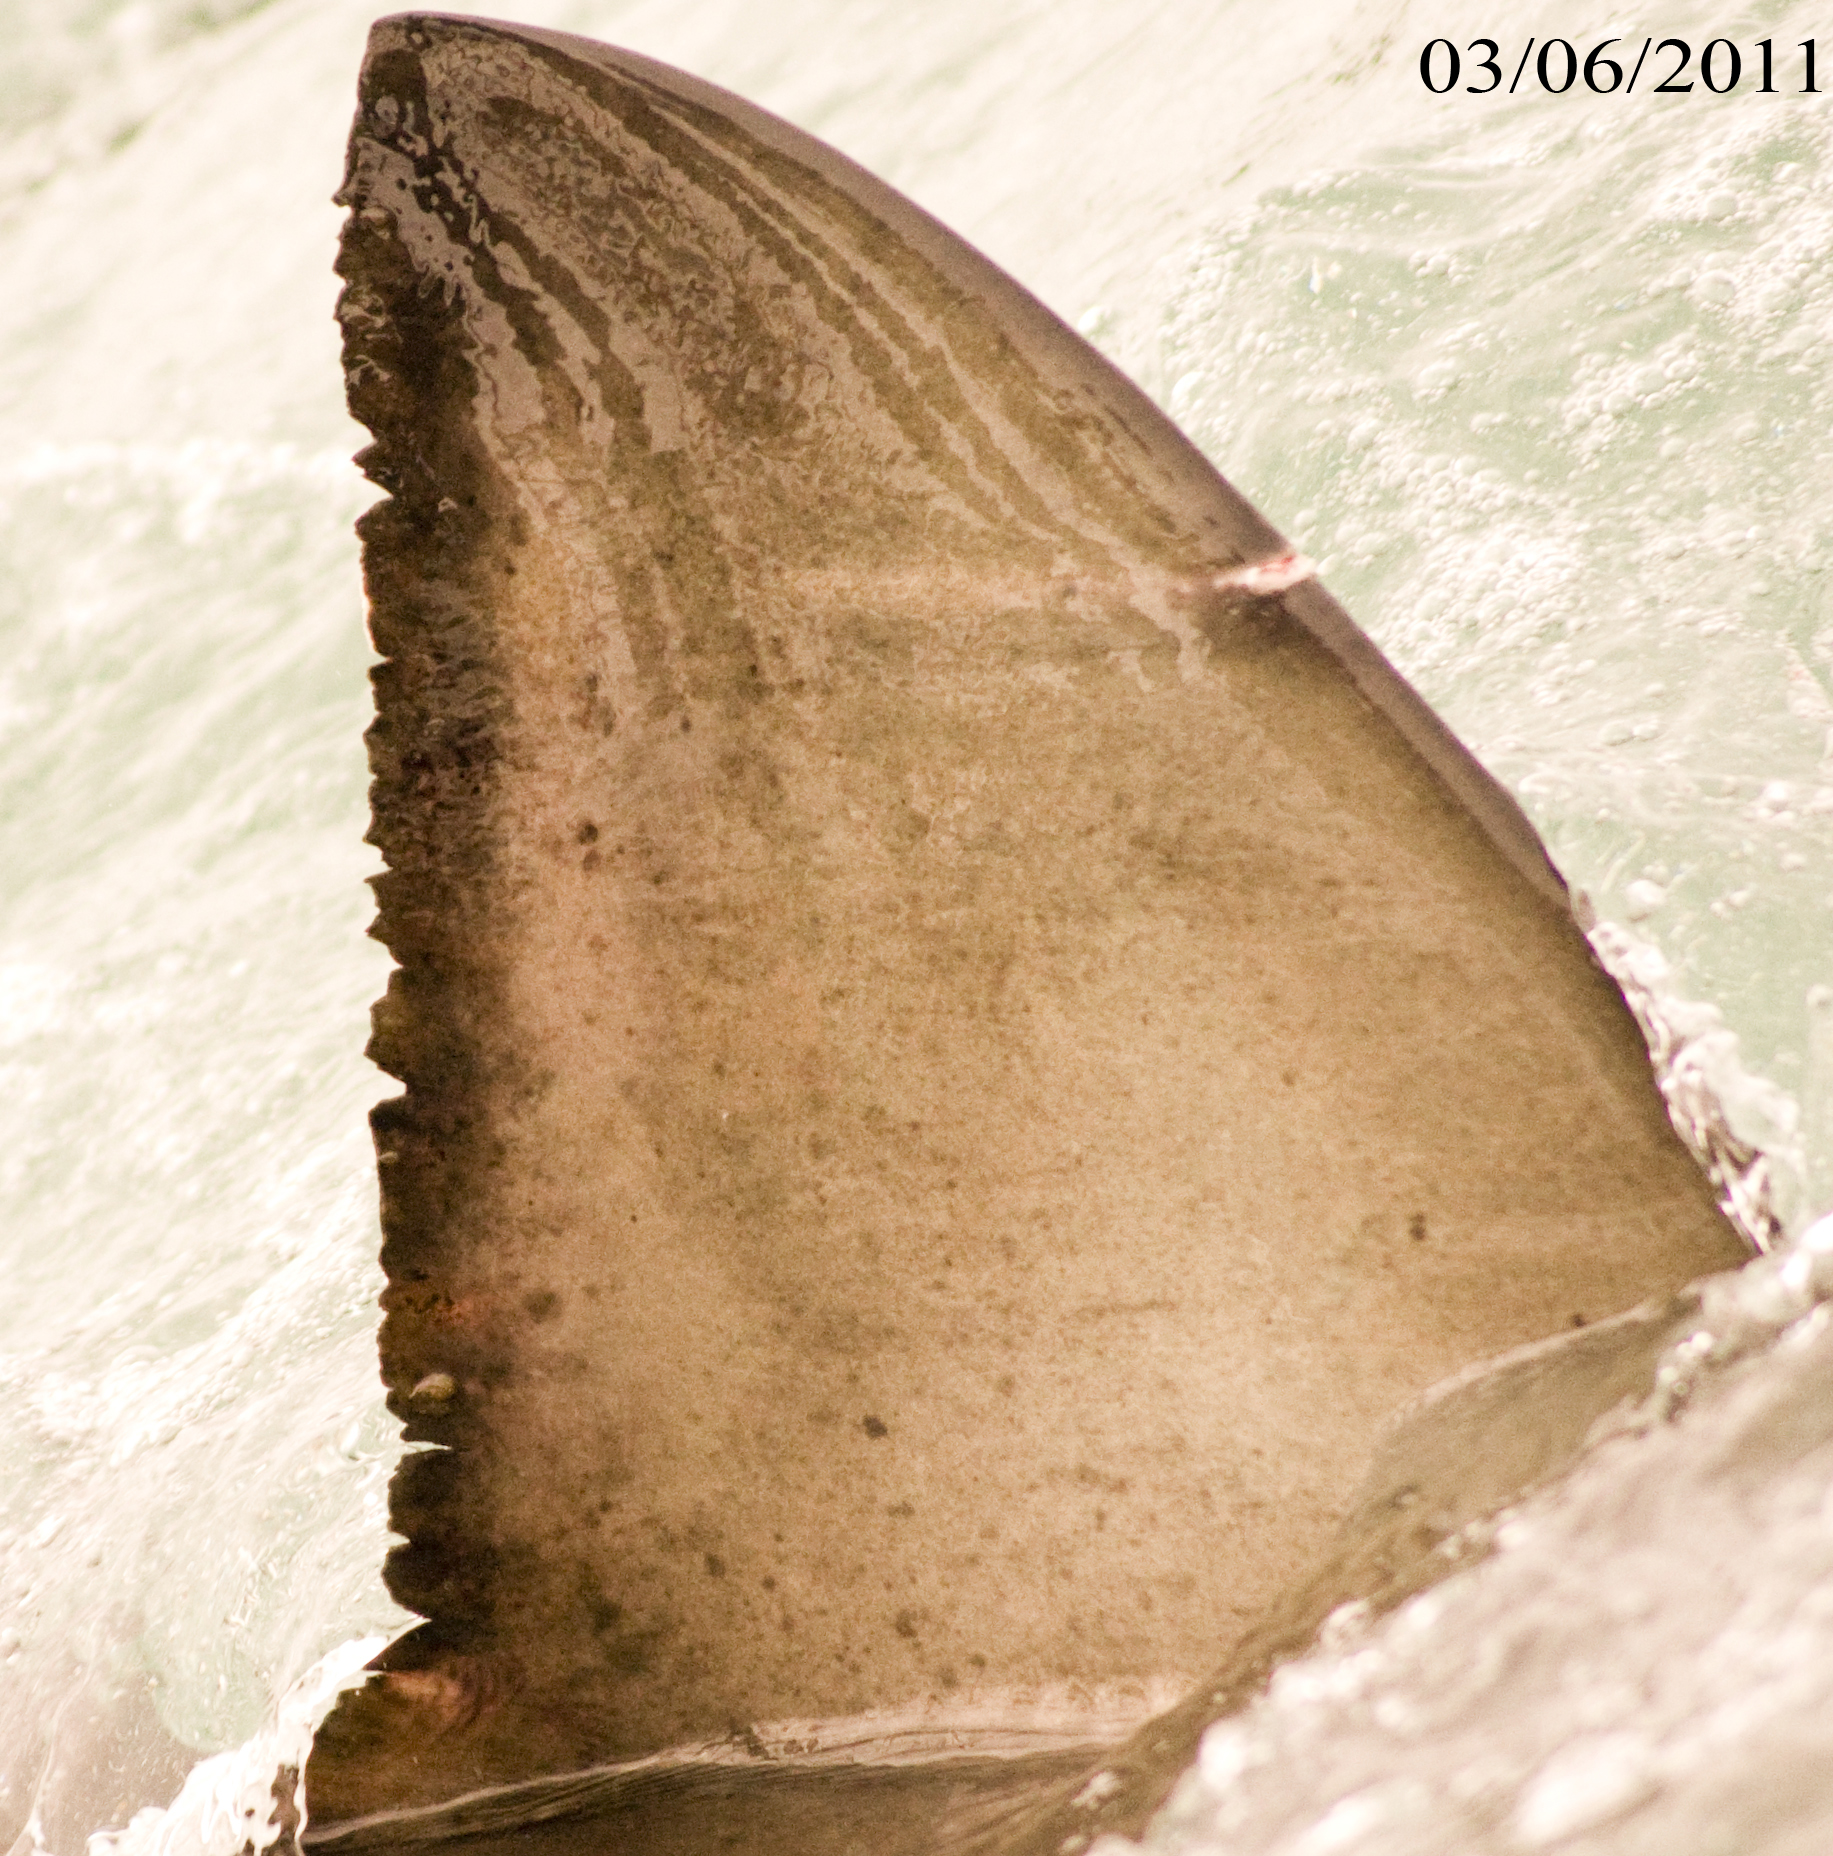
\includegraphics[width=2in]{haai3.jpg}} \quad
\subfigure[Shark fin 4]{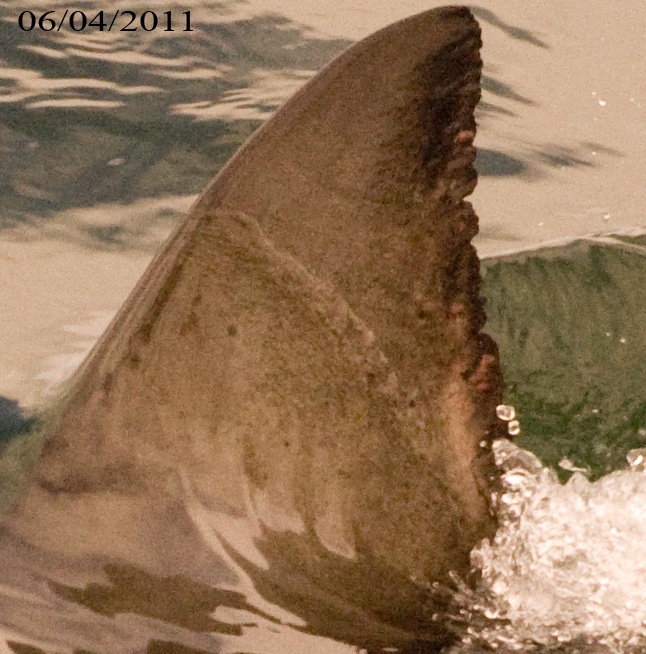
\includegraphics[width=2in]{haai4.jpg}}}
\end{figure}
\end{frame}

\begin{frame}
\frametitle{Background}
\end{frame}

\begin{frame}
\frametitle{The Grow Cut segmentation algorithm}
\end{frame}

\begin{frame}
\frametitle{}
\end{frame}

\begin{frame}
\frametitle{Algorithms from Scikit-image} 
\end{frame}

\begin{frame}
\frametitle{Current work} 
\end{frame}

\begin{frame}
\frametitle{Problems encountered}
\end{frame}

\begin{frame}
\frametitle{DARWIN}
\end{frame}

\begin{frame}
\frametitle{Conclusions}
\end{frame}

\begin{frame}
\frametitle{Future work/Objectives}
\end{frame}

\begin{frame}
\frametitle{Bibliography}
\bibliographystyle{plain}
\bibliography{beamer}
\end{frame}

\end{document}
